\section{Auswertung}
\label{sec:auswertung}

	\subsection{Versuch 501} % (fold)
	\label{sub:versuch_501}
	
	% subsection versuch_501 (end)
		
		F"ur Aufgabe 501a ergaben sich die Messwerte aus den Tabellen \ref{tabelle_1} und \ref{tabelle_2}. Die dazugeh"ohrigen Graphen sind die Graphen \ref{501a200} bis \ref{501a400}.
		Es ist zu erkennen, dass sich der Elektronenstrahl bei h"ohen Beschleunigungsspannungen $U_B$ weniger Stark abl"anken l"asst. Daraus folgt, dass auch die Empfindlichkeit $D/U_d$ mit gr"o"serem $U_B$ abnimmt. Dies ist in Tabelle \ref{tabelle_5} und dem dazugeh"origen Graphen \ref{501a}, wo die Empfindlichkeit gegen $1/U_B$ aufgetragen ist.
		Als Steigung $a$ Ausgleichsgeraden ergibt sich $a = \SI{35.848 (947)}{\centi\meter}$.
		Bei der Berechnung des Proportionalit"atsfaktors $\frac{pL}{2d}$ muss darauf geachtet werden, dass die Ablenkplatten nicht "uberall parallel zueinander liegen. Daraus folgt als Mittelwert f"ur $d$:

		\begin{eqnarray*}
			d_1 &=& \SI{0.38}{\centi \meter}\\
			\delta p_1 &=& \frac{\SI{1.03}{\centi \meter}}{\SI{1.9}{\centi \meter}}\\
			d_2 &=& \frac{\SI{0.38}{\centi \meter}+\SI{0.95}{\centi\meter}}{2}\\
			\delta P_2 &=& \frac{\SI{1.9}{\centi \meter}-\SI{1.03}{\centi\meter}}{\SI{1.9}{\centi\meter}}\\
			\Rightarrow \qquad d &=& d_1 * \delta p_1 + d_2 * \delta p_2 = \SI{26.61}{\centi\meter}
		\end{eqnarray*} 

		Somit ergibt sich f"ur $\frac{pL}{2d}$:

		\begin{eqnarray*}
			p &=& \SI{1.9}{\centi \meter}\\
			L &=& \SI{14.3}{\centi \meter}\\
			d &=& \SI{0.29}{\centi \meter}\\
			\Rightarrow \qquad \frac{pL}{2d} &=& \SI{46.84}{\centi\meter}
		\end{eqnarray*}

		F"ur Aufgabe 501b ergaben sich die Werte in der Tabelle \ref{tabelle_5}. Eine nicht lineare Regression des Graphen \ref{501a} ergab f"ur die Sinusfrequenz $\nu_{si} = \SI{79.467 (98)}{\hertz}$.
		\newpage

		\begin{table}[h]
\begin{center}
\begin{tabular}{c|c|c||c|c|c||c|c|c}
Ub[V] & Ud[V] & D[1/4 in] & Ub[V] & Ud[V] & D[1/4 in] & Ub[V] & Ud[V] & D[1/4 in] \\
\hline
200 & -7,1 & 4 & 250 & -9,3 & 4 & 300 & -11,9 & 4 \\
200 & -3,9 & 3 & 250 & -5,2 & 3 & 300 & -7,1 & 3 \\
200 & -0,1 & 2 & 250 & -0,4 & 2 & 300 & -1,2 & 2 \\
200 & 3,4 & 1 & 250 & 4 & 1 & 300 & 4,3 & 1 \\
200 & 6,9 & 0 & 250 & 8,4 & 0 & 300 & 9,5 & 0 \\
200 & 10,5 & -1 & 250 & 12,6 & -1 & 300 & 14,8 & -1 \\
200 & 13,7 & -2 & 250 & 17,3 & -2 & 300 & 20,4 & -2 \\
200 & 17,4 & -3 & 250 & 21,4 & -3 & 300 & 25,3 & -3 \\
200 & 20,7 & -4 & 250 & 25,4 & -4 & 300 & 30,0 & -4 \\
\end{tabular}
\caption{Messwerte zu Aufgabe a bei verschiedenen Beschleunigungsspannungen}
\label{tabelle_1}
\end{center}
\end{table}
		\begin{table}[h]	
\centering
\begin{tabular}{|l l||l l||l l|} \hline
	x[mm] & I[nA] & x[mm] & I[nA] & x[mm] & I[nA]\\
	\hline
	0	&	2.5   &  17	&	15  & 34	&	4.8\\
	1	&	2.1   &  18	&	13  & 35	&	3\\
	2	&	2.1   &  19	&	12.5& 36	&	1.85\\
	3	&	2.5   &  20	&	23.5& 37	&	1.55\\
	4	&	2.9   &  21	&	50  & 38	&	2.1 \\
	5	&	2.85  &  22	&	98  & 39	&	2.85\\
	6	&	2.5   &  23	&	135 & 40	&	3\\
	7	&	2.75  &  24	&	165 & 41	&	2.8\\
	8	&	4     &  25	&	155 & 42	&	1.95\\
	9	&	6.2   &  26	&	125 & 43	&	1\\
	10	&	8     &  27	&	92  & 44	&	0.6\\
	11	&	7.9   &  28	&	50  & 45	&	0.51\\
	12	&	6     &  29	&	25.5& 46	&	0.72\\
	13	&	4     &  30	&	11  & 47	&	0.86\\
	14	&	4.8   &  31	&	7.2 & 48	&	0.86\\
	15	&	8.5   &  32	&	6.4 & 49	&	0.68\\
	16	&	13    &  33	&	6   & 50	&	0.45\\
	\hline
\end{tabular}
\caption{Intensit"at des festen Einfachspalts abgh"angig von der Detektorstellung x}
\label{tabelle_2}
\end{table}



		\begin{figure}[htbp]
			\centering
			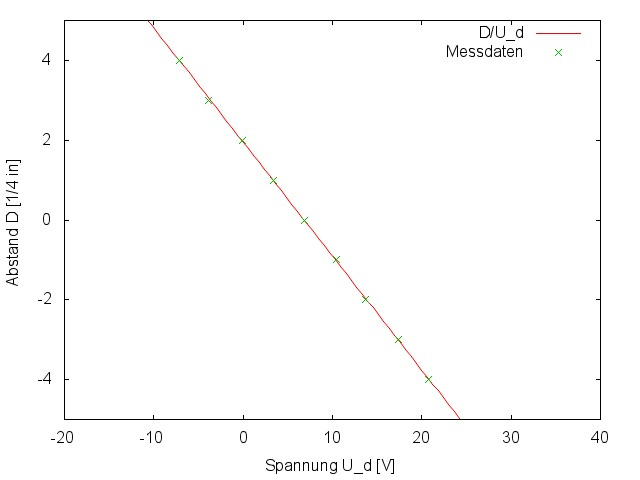
\includegraphics[width = 12cm]{img/501a200.jpg}
			\caption{Messergebniss zu a bei $U_B = 200$}
			\label{501a200}
		
			\centering
			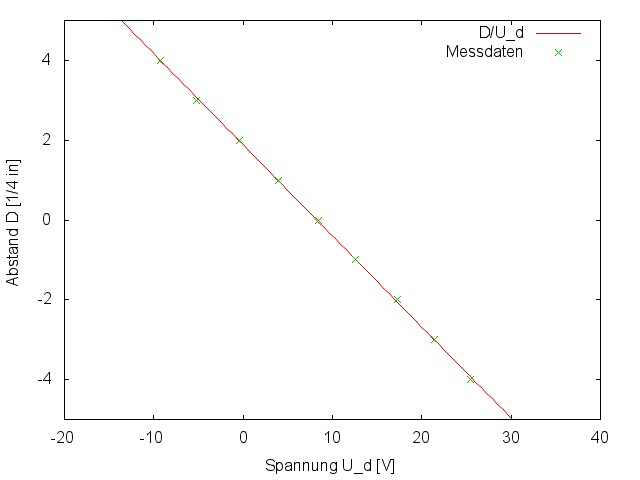
\includegraphics[width = 12cm]{img/501a250.jpg}
			\caption{Messergebniss zu a bei $U_B = 250$}
			\label{501a250}
		\end{figure}
		\begin{figure}[htbp]
			\centering
			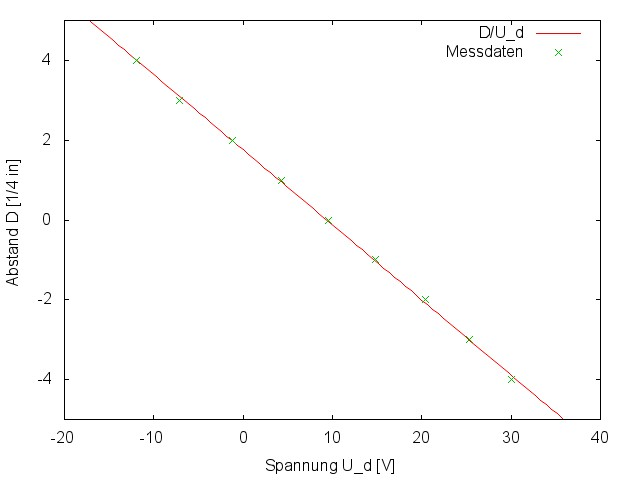
\includegraphics[width = 12cm]{img/501a300.jpg}
			\caption{Messergebniss zu a bei $U_B = 300$}
			\label{501a300}
		
			\centering
			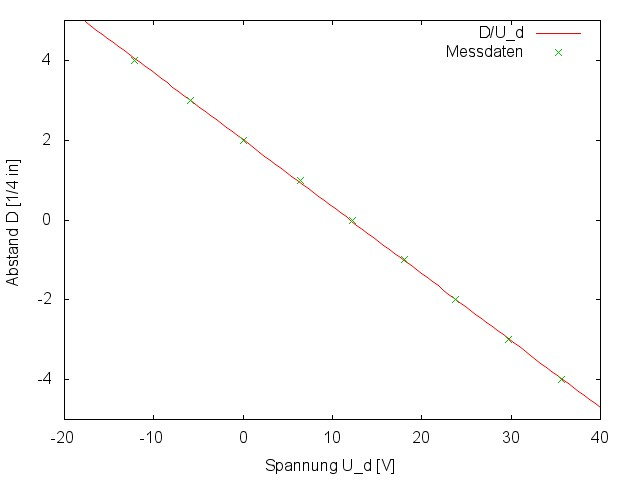
\includegraphics[width = 12cm]{img/501a350.jpg}
			\caption{Messergebniss zu a bei $U_B = 350$}
			\label{501a350}
		\end{figure}
		\begin{figure}[htbp]
			\centering
			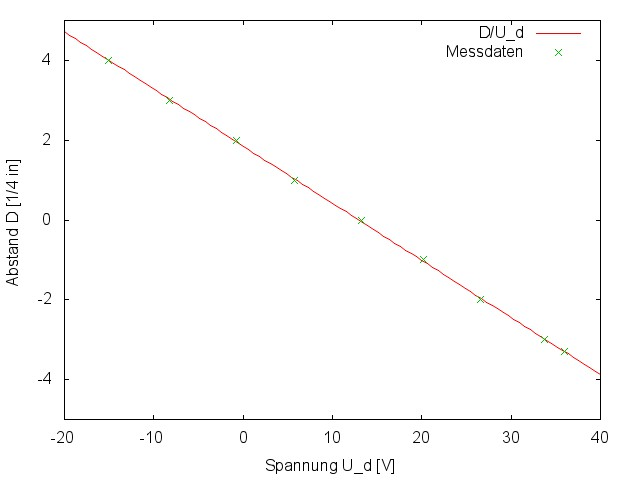
\includegraphics[width = 12cm]{img/501a400.jpg}
			\caption{Messergebniss zu a bei $U_B = 400$}
			\label{501a400}
		\end{figure}

		\begin{table}
\begin{center}
\begin{tabular}{c|c}
a[cm/V] & 1/Ub[1/V] \\
\hline
-0.286 & 1/200 \\
-0.228 & 1/250 \\
-0.188 & 1/300 \\
-0.168 & 1/350 \\
-0.143 & 1/400 \\
\end{tabular}
\caption[]{Empfindlichkeit von D/Ud gegen 1/Ub}
\label{tabelle_5}
\end{center}
\end{table}

		\begin{figure}[h]
			\centering
			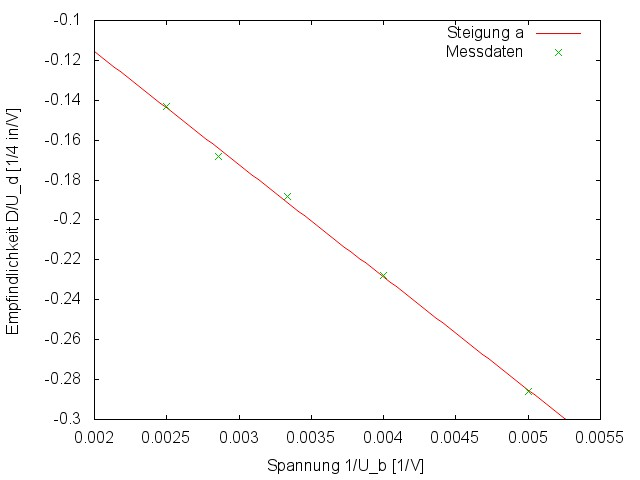
\includegraphics[width = 12cm]{img/501a.jpg}
			\caption{Empfindlichkeit von D/Ud gegen 1/Ub}
			\label{501a}
		\end{figure}

		\begin{table}[h]	
\centering
\begin{tabular}{|l l||l l||l l|} \hline
	x[mm] & I[nA] & x[mm] & I[nA] & x[mm] & I[nA]\\
	\hline
	0	&	1     &  17	&	6.4   & 34	&	2.8\\
	1	&	2.3   &  18	&	25    & 35	&	10\\
	2	&	1.6   &  19	&	8     & 36  &	2.8\\
	3	&	1.4   &  20	&	26    & 37  &	3.4\\
	4	&	0.98  &  21	&	24    & 38	&	2.9\\
	5	&	0.6   &  22	&	12.5  & 39	&	0.66\\
	6	&	0.78  &  23	&	38    & 40	&	1.25\\
	7	&	0.36  &  24	&	9.4   & 41	&	0.38\\
	8	&	0.58  &  25	&	32    & 42	&	0.34\\
	9	&	0.53  &  26	&	22.5  & 43	&	0.36\\
	10	&	1.25  &  27	&	17    & 44	&	0.3\\
	11	&	2.25  &  28	&	32    & 45	&	0.5\\
	12	&	1.6   &  29	&	6.8   & 46	&	0.5\\
	13	&	7     &  30	&	28    & 47	&	0.68\\
	14	&	3.2   &  31	&	10.5  & 48	&	0.68\\
	15	&	9.6   &  32	&	10.5  & 49	&	0.64\\
	16	&	12.5  &  33	&	16    & 50	&	0.77\\
	\hline
\end{tabular}
\caption{Intensit"at des festen Doppelspalts abgh"angig von der Detektorstellung x}
\label{tabelle_3}
\end{table}



		\begin{figure}[htbp]
			\centering
			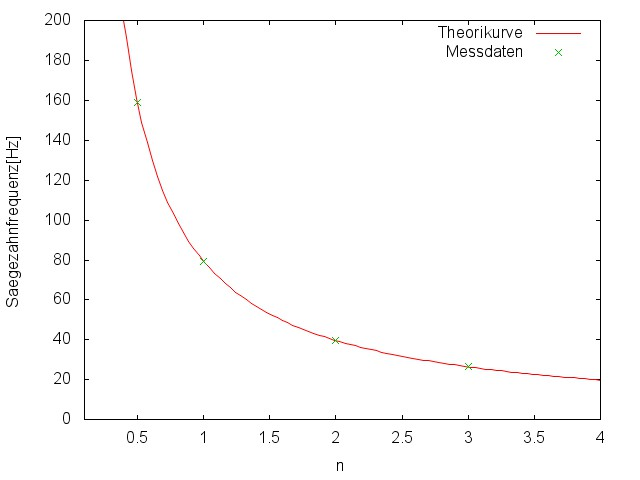
\includegraphics[width = 12cm]{img/501b.jpg}
			\caption{n-Fache der S"agezahnspannung}
			\label{501b}
		\end{figure}

		\newpage

	\subsection{Versuch 502} % (fold)
	\label{sub:versuch_502}
		
		In Aufgabenteil 502a ergab sich f"ur die Ausgleichsrechnug der Daten aus Tabelle \ref{tabelle_4}, mithilfe der Graphen \ref{502a250} und \ref{502a450}, ergab:

		\begin{eqnarray*}
			L &=& \SI{17.3}{\centi\meter}\\
			N &=& 20\\
			R &=& \SI{0.282}{\meter}\\
			B &=& \mu_0 \frac{8}{\sqrt{125}} \frac{NI}{R} = 6.377*10^{-5}*I\,\SI{}{\tesla}\\
			\Rightarrow\\
			a &=& \SI{9756.13 (14810)}{1\per\meter\tesla}\\
			b &=& \SI{7281.19 (7729)}{1\per\meter\tesla}
		\end{eqnarray*}

		Mit Hilfe der Proportionalit"atsfaktoren $a, b$ und der Gleichung $a, b = \sqrt{\frac{e_0}{8 U_B m_0}}$ ergibt sich f"ur die spezifische Ladung der Elektronen:

		\begin{eqnarray*}
			\frac{e_0}{m_0} &=& 8*\SI{250}{\volt}*(\SI{9756.13 (14810)}{1\per\meter\tesla})^2 = \SI{1.936}{\coulomb\per\kilo\gram}*10^{11}\\
			\frac{e_0}{m_0} &=& 8*\SI{450}{\volt}*(\SI{7281.19 (7729)}{1\per\meter\tesla})^2 = \SI{1.909}{\coulomb\per\kilo\gram}*10^{11}
		\end{eqnarray*}

		F"ur Aufgabenteil 502b ergab sich bei einer Beschleunigungsspannung $U_B = \SI{200 (5)}{\volt}$ f"ur den Ausgleichsstorm ein Wert von $\SI{0.26}{\ampere}$. Die Messung des Inklinationswinkels ergab $\varphi = 70$ Grad. Daraus folgt f"ur das Erdmagnetfeld:

		\begin{eqnarray*}
			B_\mathrm{hor} &=& 6.377*10^{-5}*I\,\SI{}{\tesla} = \SI{16.58}{\micro\tesla}\\
			\Rightarrow \qquad B_\mathrm{total} &=& \frac{B_{hor}}{\cos(\varphi)} = \SI{48.48}{\micro\tesla}
		\end{eqnarray*}


		\newpage

		\begin{table}
\begin{center}
\begin{tabular}{c|c|c||c|c|c}
Ub[V] & I[A] & D[1/4 in] & Ub[V] & I[A] & D[1/4 in] \\
\hline
250 & 0 & 4 & 450 & 0 & -4 \\
250 & 0,28 & 3 & 450 & 0,5 & -3 \\
250 & 0,7 & 2 & 450 & 0,95 & -2 \\
250 & 0,9 & 1 & 450 & 1,4 & -1 \\
250 & 1,3 & 0 & 450 & 1,8 & 0 \\
250 & 1,6 & -1 & 450 & 2,25 & 1 \\
250 & 1,95 & -2 & 450 & 2,7 & 2 \\
250 & 2,3 & -3 & 450 & 3,15 & 3 \\
250 & 2,6 & -4 & 450 & 3,3 & 3,5 \\
\end{tabular}
\caption{Messwerte zu 502b, vor dem Aufnehmen der rechten Daten hat eine Umpolung stattgefunden}
\label{tabelle_4}
\end{center}
\end{table}


		\begin{figure}[h]
			\centering
			\includegraphics[width = 14cm]{img/502a250.jpg}
			\caption{Graph zur Berechnung des Proportionalit"atsfaktors a}
			\label{502a250}

			\includegraphics[width = 14cm]{img/502a450.jpg}
			\caption{Graph zur Berechnung des Proportionalit"atsfaktors b}
			\label{502a450}
		\end{figure}		

		\newpage